\documentclass[conference]{IEEEtran}
\IEEEoverridecommandlockouts
% The preceding line is only needed to identify funding in the first footnote. If that is unneeded, please comment it out.
%Template version as of 6/27/2024

\usepackage{cite}
\usepackage{float}
\usepackage{amsmath,amssymb,amsfonts}
\usepackage{algorithmic}
\usepackage{graphicx}
\usepackage{textcomp}
\usepackage{xcolor}
\def\BibTeX{{\rm B\kern-.05em{\sc i\kern-.025em b}\kern-.08em
    T\kern-.1667em\lower.7ex\hbox{E}\kern-.125emX}}
\begin{document}

\title{YZV 202E Optimization for Data Science Project Proposal Efficient Selection of Green Space Locations in Istanbul Project Report}

\author{\IEEEauthorblockN{Yusuf Solmaz}
\IEEEauthorblockA{\textit{Computer and Informatics Department} \\
\textit{Istanbul Technical University}\\
solmaz22@itu.edu.tr \\
150220306}
\and
\IEEEauthorblockN{Necip Fazıl Doğan}
\IEEEauthorblockA{\textit{Computer and Informatics Department} \\
\textit{Istanbul Technical University}\\
doganne23@itu.edu.tr \\
150230311}
\and
\IEEEauthorblockN{İbrahim Bancar}
\IEEEauthorblockA{\textit{Computer and Informatics Department} \\
\textit{Istanbul Technical University}\\
bancar22@itu.edu.tr \\
150220313}
}

\maketitle

\begin{abstract}
This report analysis Efficient Selection of Green Space Locations in Istanbul project. The project aims spread green space over Istanbul using Genetic Algorithm and Particle Swarm Optimization. Current green space size, population, air quality and transportation accessibility conditions considered in county determination process. The objective function aims to improve the state of life with balance of these factors. The objective function has also cost constraints. The report analysis convergence success of PSO and GA. Also, the report examines reaction of objective function under different weights. 
\end{abstract}

\section{Problem Description}
Green spaces are very important for quality of life, sustainability and public health. In metropolis like Istanbul, the population increases and urban sprawl causes green spaces to spread inefficiently. As a result, air pollution increases, heat distribution affects negatively and like this problem. These problems have negative effects on public health.\\
The project aims determine new green space locations and sizes based on population, air quality, current green spaces and transportation accessibility. Main problem is determination of county need green spaces and how much size under cost constraints. 

\section{Method Formulation}
\subsection{Data Collection and Process}
\begin{itemize}
    \item Current Green Space\\
    Data including current green space information as geojson file gathered from official IBB website. This data processed for split data with respect to counties and total green space. Final data includes total green space area for each county.
    \item Population\\
    Population data is collected from IBB website and categorized each counties population
    \item Air Quality\\
    Air quality data is collected from IBB api. AQI scores are saved hourly for all days between 2024-2025 from 28 air quality  measurement center. Each center takes average of the yearly AQI value. Rest of counties take value from the closest center.
    \item Public Transportation\\
    Number of railway, minibus and taxi stations are gathered from IBB dataset. These stations are weighed in support of railway more to determine transportation score for all counties.
\end{itemize}
\subsection{Objective Function}
$$\text{Minimize }f(x)=\sum_i^n\frac{(W_1\cdot AQI_{i,norm}+W_2\cdot T_{i,norm})P_i}{GS_i+x_i+\epsilon}$$
AQI: Air Quality Index\\
T: Transportation Score\\
P: Population\\
GS: Current Green Space\\
x: New Green Space\\
AQI and T values are used under linear normalization. $\epsilon$ value is for avoiding divided by zero error.\\
Objective function give sum of the all counties performance value. This value has negative correlation with new and current green space size. Also, this value increase with respect to air quality, transportation and population scores. To minimize this function, the x values become larger with respect to the other parameters. $W_1$ and $W_2$ weights determine which parameter is more important between air quality and transportation. Penalty is used for county exceed the constraints.
\subsection{Constraints}
\begin{itemize}
    \item Total Green Space Limit\\
    $$\sum_{i=0}^nx_i \leq 3,000,000$$
    This constrain is for prevent exceeding cost limit with too much rising of green space
    \item County Green Space Limit
    $$x_i\leq 0.5\cdot GS_i$$
    This constraint is for prevent concentrating some counties and, giving too much green space there.
    \item Positive Space
    $$x_i \geq 0$$
    This constraint is for prevent negative space for right result.
\end{itemize}
\subsection{Optimization Algortihms}
\subsubsection{Genetic Algorithm}
New green space vector x is used as chromosome in GA.
\begin{itemize}
    \item Create Population\\
    A random value under the constraint is generated for each county.
    \item Mutation\\
    20\% mutation probability are applied for each chromosome.
    \item Crossover\\
    Selected 2 parents are crossover with alpha method which is $child=\alpha\cdot parent_1+(1-\alpha)\cdot parent_2$
    \item Selection\\
    Best 10\% of the population pass the next generation.
\end{itemize}
\subsubsection{Particle Swarm Optimization}
\begin{itemize}
    \item Initialize Particles\\
    Each particle get random x and v values.
    \item Update Velocities\\
    Each particle update own velocity between individual best and group best.
\end{itemize}

\section{Real-World Application}
Urban planning departments of large municipalities like Istanbul can utilize this type of optimization framework to make data-driven decisions regarding land use and environmental equity. By integrating dynamic variables such as air quality and transportation accessibility, the model ensures that future green area investments are both fair and impactful. This approach can also be generalized to other resource allocation problems in urban planning.


\section{Experimental Evaluation}
Optimization algorithms are applied with different weights. Next results are equal weighted transportation and air quality unless otherwise stated
\subsection{Comparison of 2 Methods}
\begin{figure}[H]
    \centering
    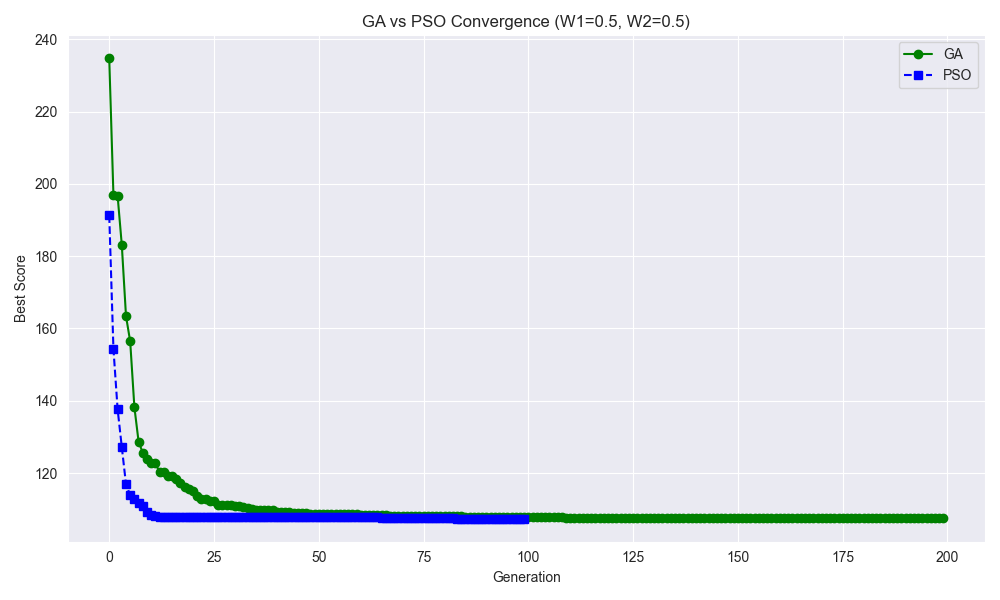
\includegraphics[width=0.8\linewidth]{ga_vs_pso_convergence.png}
    \caption{Comparison of 2 Methods}
    \label{fig:compare}
\end{figure}
GA and PSO give different results for different seed values, but in general, it can be seen that GA gives slightly better results than PSO. In addition, when looking at the graph below, it can be said that PSO converges much faster than GA.

\subsection{Green Area Results by District}

The graphs below show the amount of green space per capita before adding green space and how much green space the PSO and GA provide for each district per capita.

\begin{figure}[H]
    \centering
    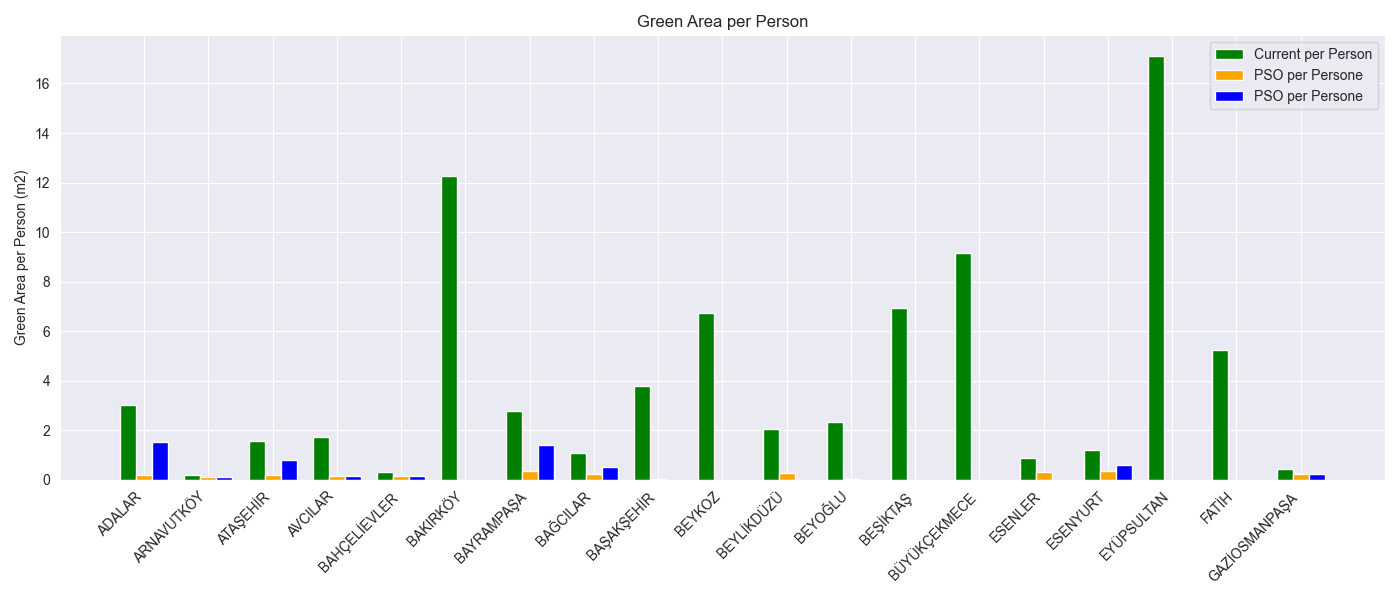
\includegraphics[width=1.0\linewidth]{group1.png}
    \caption{Green Area Results by District}
    \label{fig:green_areas_per_capita_1}
\end{figure}

\begin{figure}[H]
    \centering
    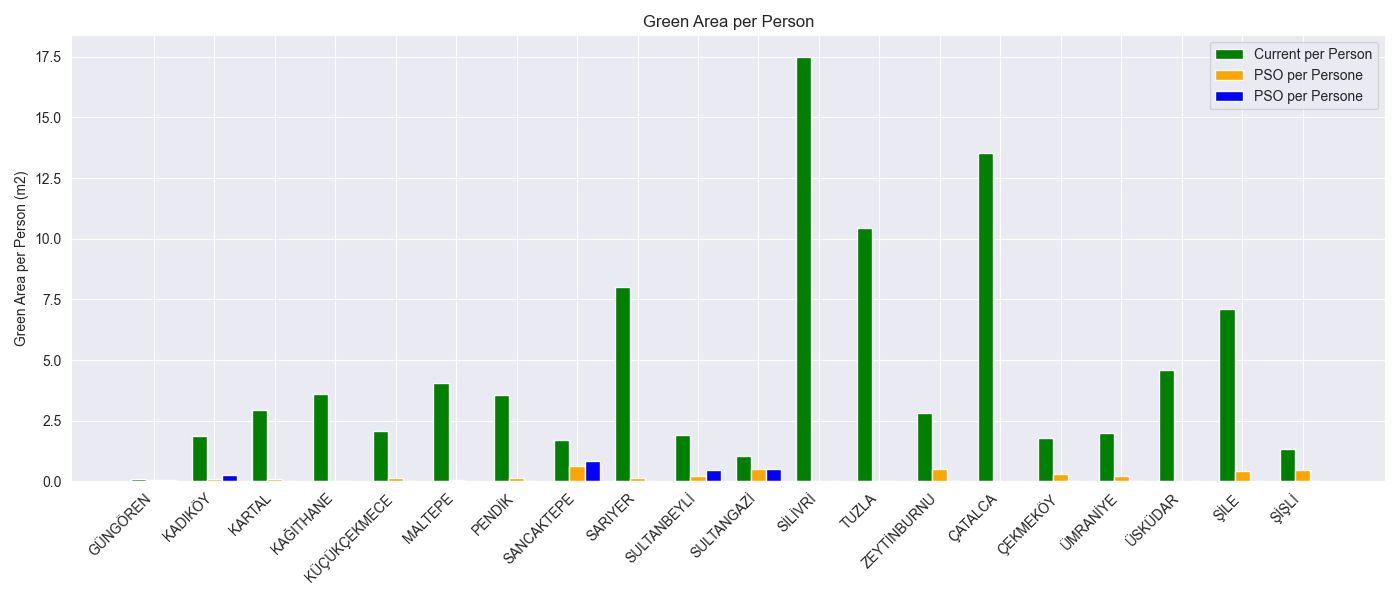
\includegraphics[width=1.0\linewidth]{group2.png}
    \caption{Green Area Results by District}
    \label{fig:green_areas_per_capita_2}
\end{figure}

Looking at the graphs above, it can be seen that both algorithms provide more green space per person in regions with less green space per person.\\

When we examine how the two algorithms distribute green areas to the districts, we see that GA distributes green areas to the entire map, while PSO distributes all green areas to a few districts and does not give any green areas to other districts. The green area distributions of GA and PSO are shown on the map in the images below.

\begin{figure}[H]
    \centering
    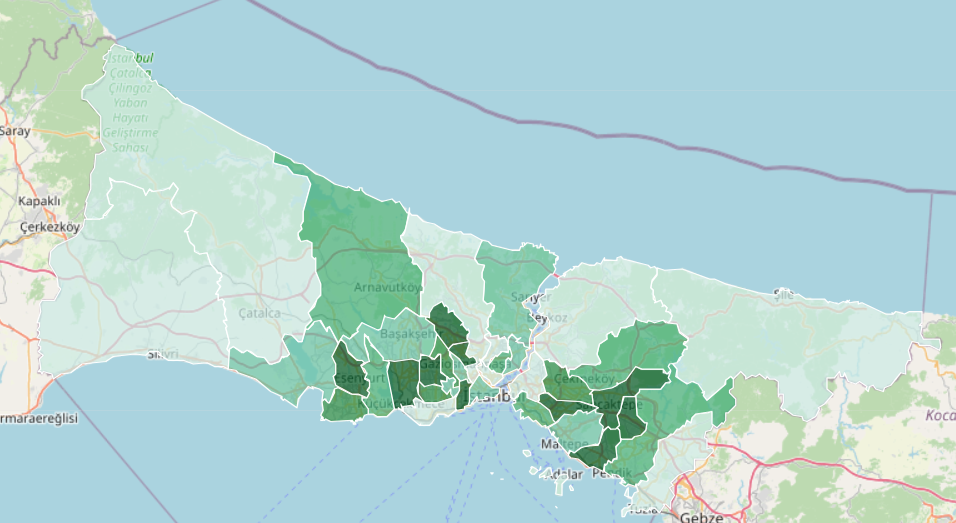
\includegraphics[width=0.8\linewidth]{map_ga.png}
    \caption{Green Area Distribution by Districts for GA}
    \label{fig:map_ga}
\end{figure}

\begin{figure}[H]
    \centering
    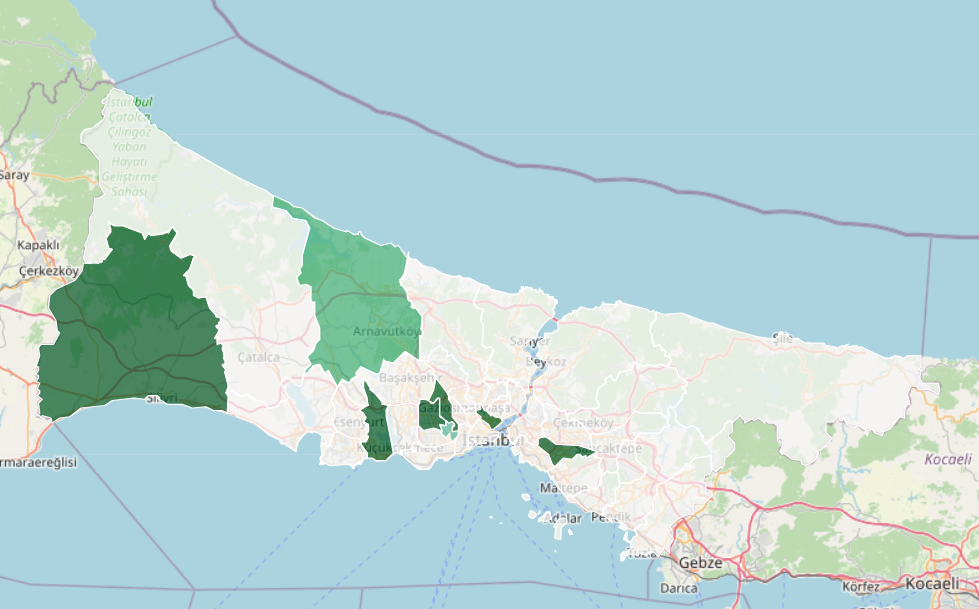
\includegraphics[width=0.8\linewidth]{map_pso.png}
    \caption{Green Area Distribution by Districts for PSO}
    \label{fig:map_pso}
\end{figure}

\section{Effect of W1 and W2 Values on Distributions}
When the objective function is examined, it is expected that the W1 value will provide more green areas to districts where air quality is poor and the W2 value will provide more green areas to districts where transportation is easy. However, when the W1 and W2 values are increased or decreased, instead of this expected result, both algorithms behave more randomly.
Despite this, it is seen that the behavior of concentrating on certain areas is more frequent in scenarios where one of the W1 and W2 values is high and the other is low, but this does not create a clear pattern.\\

In addition, it is seen that the increase in the W2 value generally causes the best scores to increase, which is the aim of the algorithms to minimize this.

\section{Conclusion}
In this study, the issue of fair and effective allocation of green spaces across the districts of Istanbul was addressed by incorporating multiple real-world factors, including population,existing green areas, air quality, and accessibility to public transportation.

Two heuristic optimization methods, Particle Swarm Optimization (PSO) and Genetic Algorithm (GA), were applied and compared under the same circumstances in order to address this issue. While GA gives slightly better results than PSO, it is seen that PSO converges much faster. When we look at the behavior of the algorithms, we see that GA provides green areas to a wider region, while PSO concentrates on some areas.

Additionally, it was examined how sensitive the objective function was to the weighting parameters W1 and W2, which stand for the respective significance of accessibility to transportation and air quality. It was discovered that imbalances in the weight arrangement frequently resulted in more polarized allocation outcomes, even though totally predictable behavior was not always seen.

This study demonstrates how heuristic optimization techniques can be applied to solve challenging urban planning issues while taking practical limitations into account. The suggested approach offers a data-driven framework that could help policymakers support sustainable development and environmental fairness in urban areas. Future work may focus on the integration of temporal planning models, stakeholder preferences, or real-time data to further enhance the model’s applicability.

\end{document}
